\section{Dataset Details}
\label{appendix:dataset_details}

\subsection{Data Distribution}
\label{appendix:data_distribution}

\begin{figure}[htbp]
    \centering
    %=========== ROW 1: CVPR 2025 =========
    \begin{subfigure}[b]{0.32\textwidth}
        \centering
        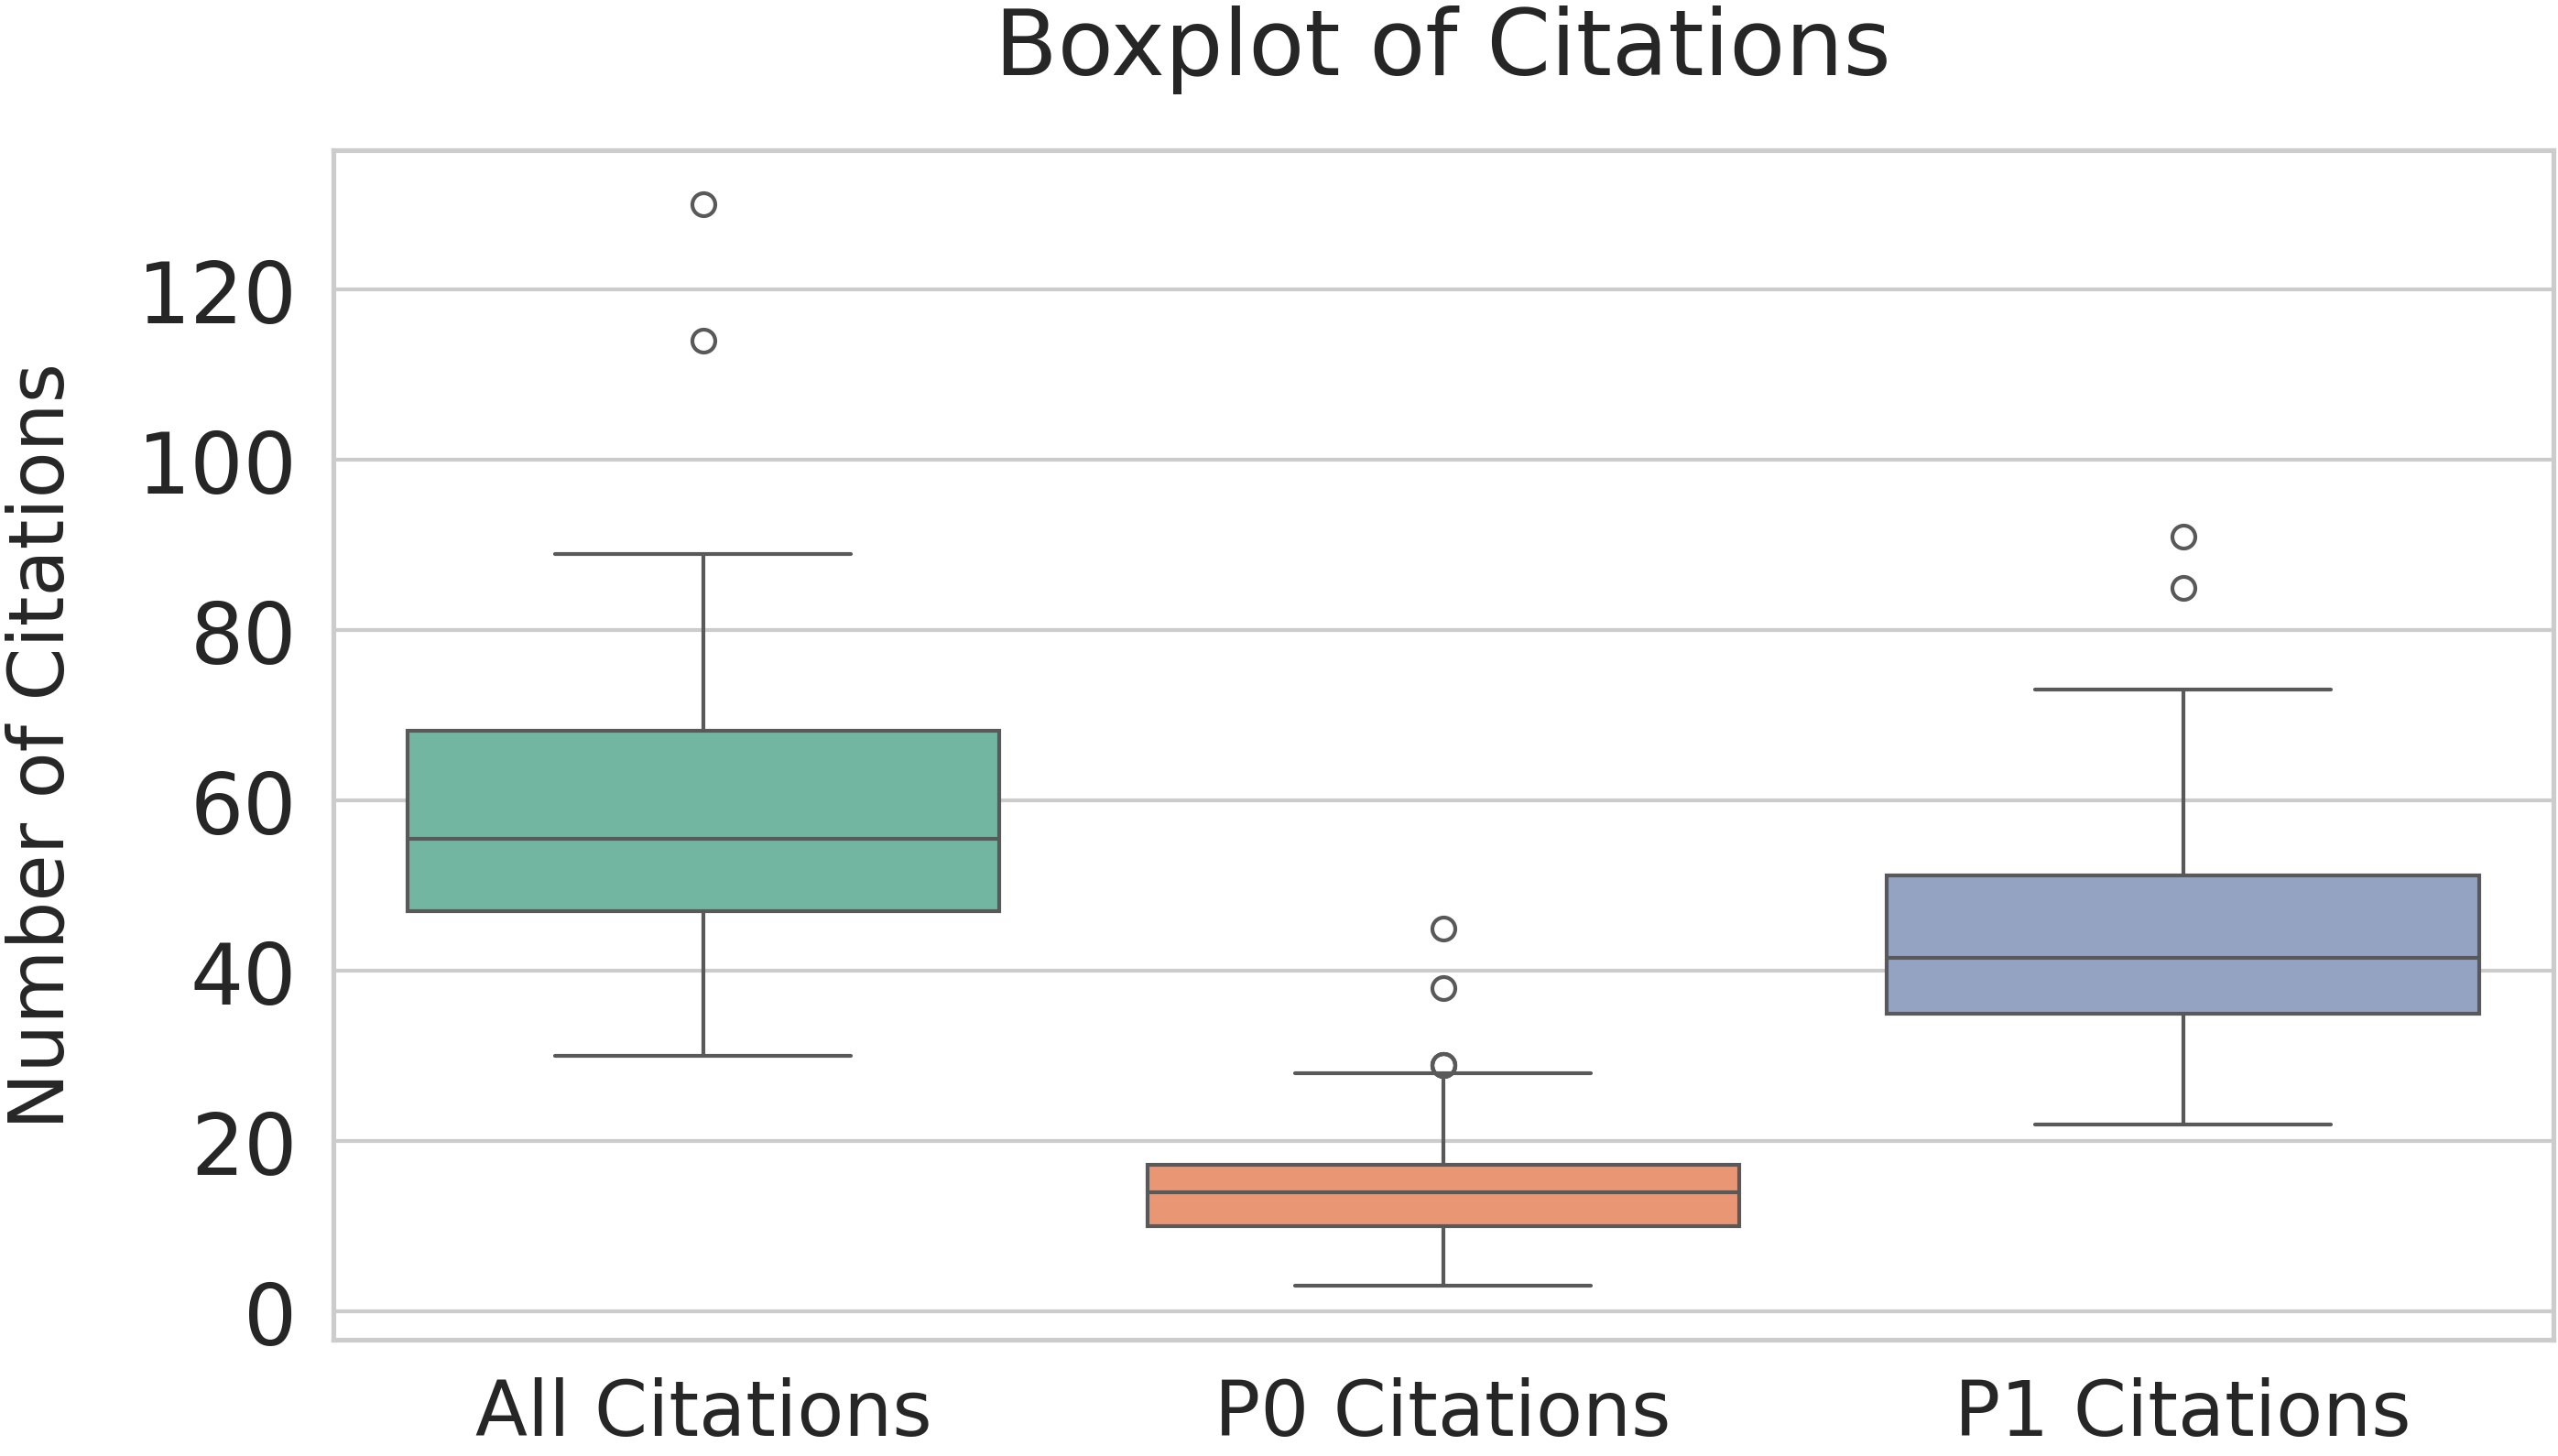
\includegraphics[width=\linewidth]{content/figures/cvpr2025_analysis/citations_boxplot.png}
        \caption{Citation Count Distribution}
    \end{subfigure}
    \hfill
    \begin{subfigure}[b]{0.32\textwidth}
        \centering
        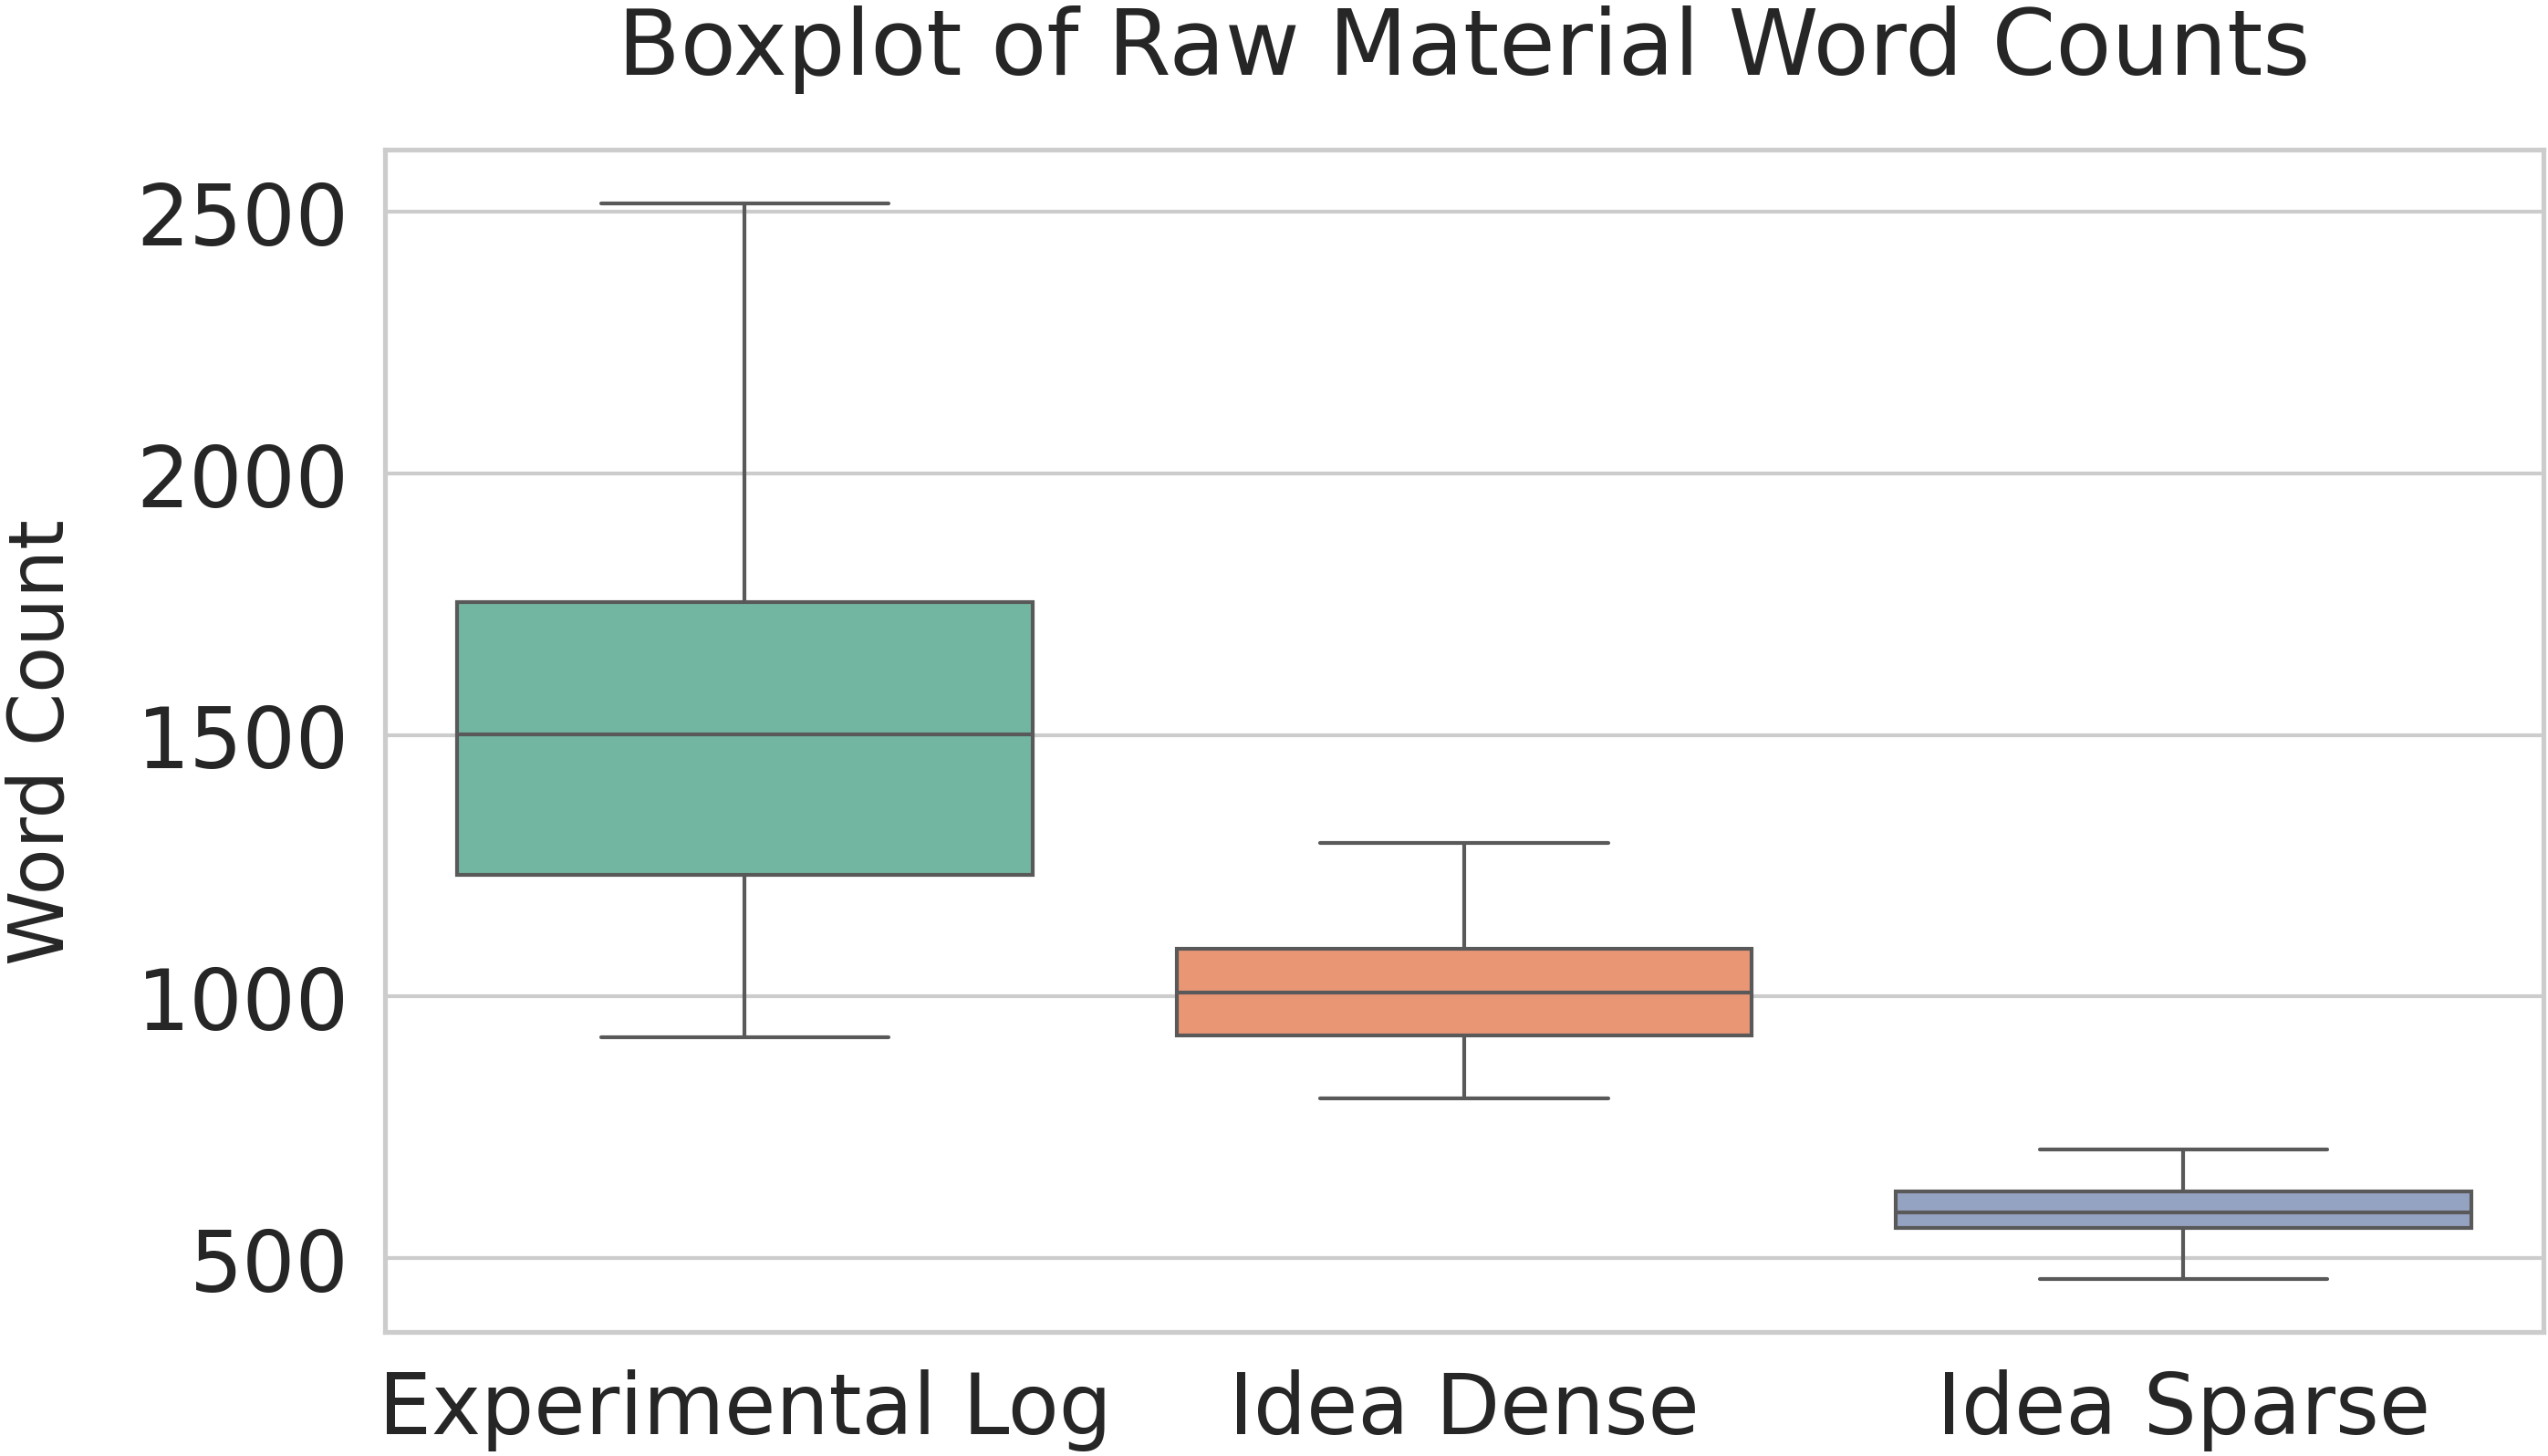
\includegraphics[width=\linewidth]{content/figures/cvpr2025_analysis/lengths_boxplot.png}
        \caption{Material Length Distribution}
    \end{subfigure}
    \hfill
    \begin{subfigure}[b]{0.32\textwidth}
        \centering
        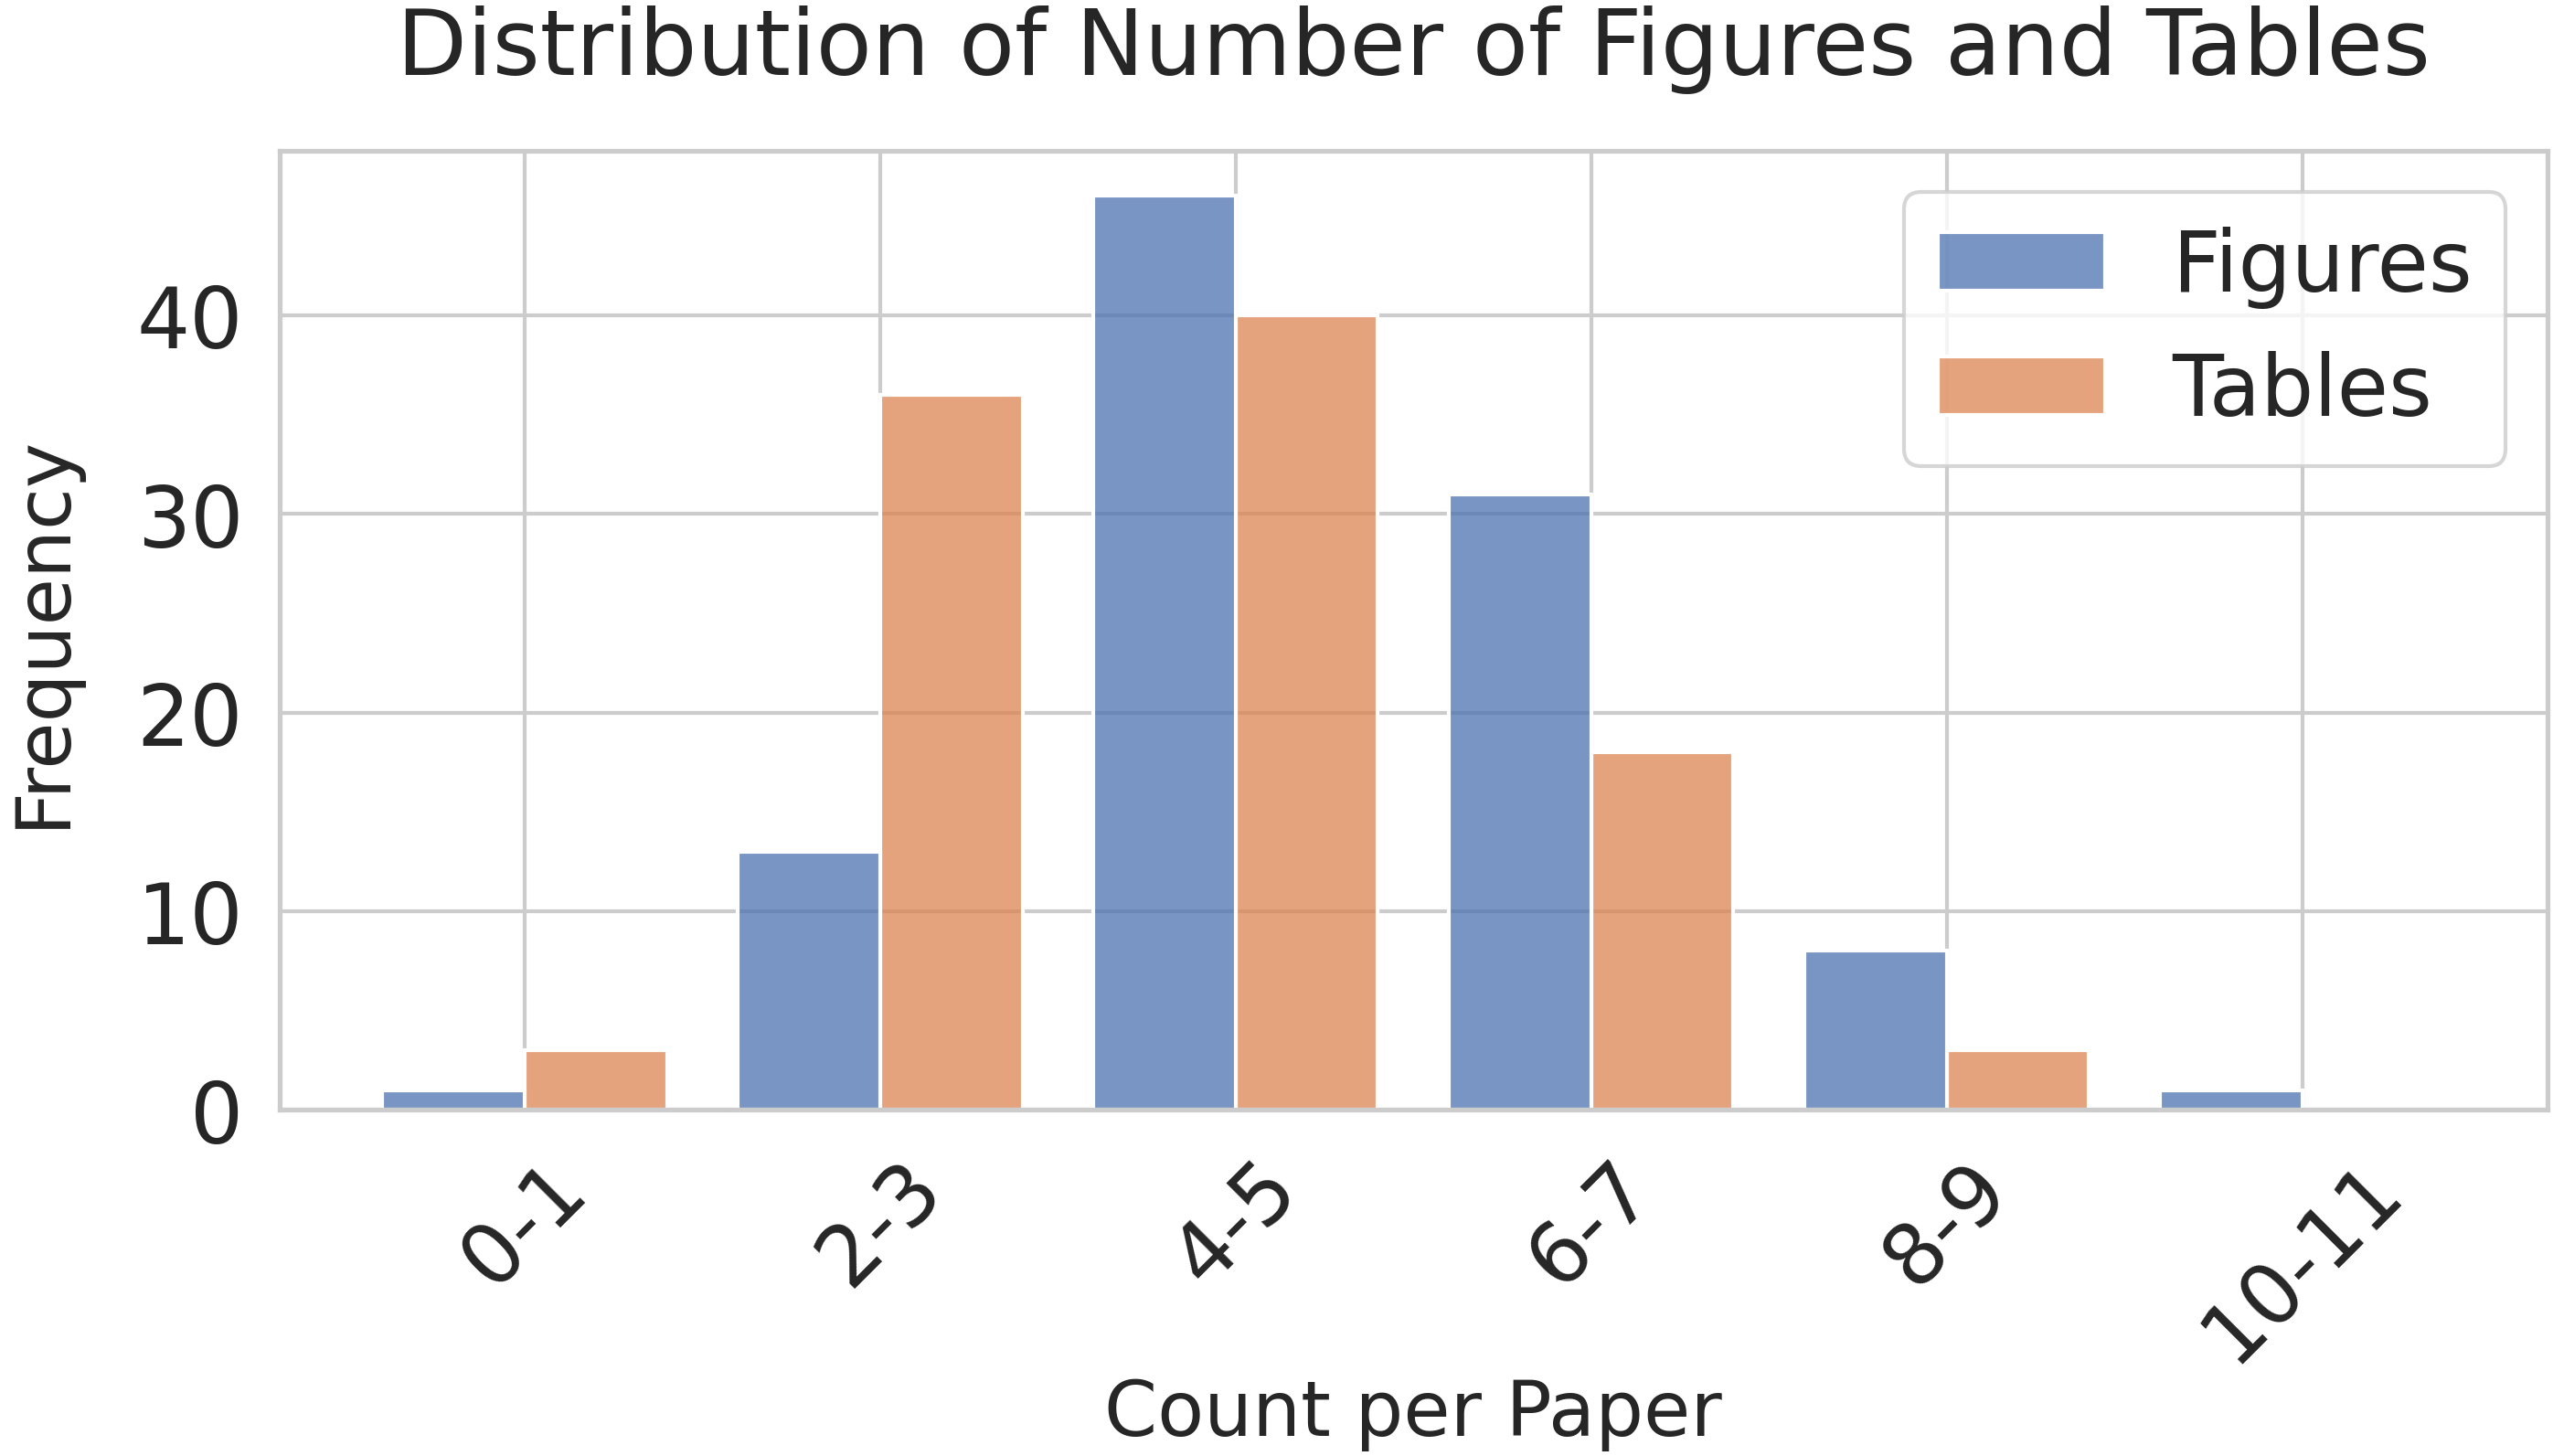
\includegraphics[width=\linewidth]{content/figures/cvpr2025_analysis/num_figures_and_tables_dist.png}
        \caption{Tables/Figures Distribution}
    \end{subfigure}
    
    \caption{CVPR 2025 Dataset Statistics}
    \label{fig:cvpr2025_distribution}
\end{figure}

\begin{figure}[htbp]
    \centering
    % ========= ROW 2: ICLR 2025 ===========
    \begin{subfigure}[b]{0.32\textwidth}
        \centering
        
\includegraphics[width=\linewidth]{content/figures/iclr2025_analysis/citations_boxplot.png}
        \caption{Citation Count Distribution}
    \end{subfigure}
    \hfill
    \begin{subfigure}[b]{0.32\textwidth}
        \centering
        
\includegraphics[width=\linewidth]{content/figures/iclr2025_analysis/lengths_boxplot.png}
        \caption{Material Length Distribution}
    \end{subfigure}
    \hfill
    \begin{subfigure}[b]{0.32\textwidth}
        \centering
        
\includegraphics[width=\linewidth]{content/figures/iclr2025_analysis/num_figures_and_tables_dist.png}
        \caption{Tables/Figures Distribution}
    \end{subfigure}
    \caption{ICLR 2025 Dataset Statistics}
    \label{fig:iclr2025_distribution}
\end{figure}

\begin{table}[h]
\centering
\resizebox{0.75\linewidth}{!}{
\begin{tabular}{lcc}
\toprule
\textbf{Metric} & \textbf{CVPR 2025} & \textbf{ICLR 2025} \\
\midrule
\textit{Visual Elements} & & \\
Number of Figures & 5.20 $\pm$ 1.73 & 9.19 $\pm$ 5.39 \\
Number of Tables & 4.20 $\pm$ 1.65 & 8.13 $\pm$ 5.19 \\
\midrule
\textit{Citations} & & \\
Total Citations & 58.52 $\pm$ 17.55 & 59.18 $\pm$ 20.01 \\
P0 Citations (must-cite) & 14.86 $\pm$ 6.72 & 13.65 $\pm$ 5.57 \\
P1 Citations (good-to-cite) & 43.66 $\pm$ 13.43 & 45.53 $\pm$ 17.36 \\
\midrule
\textit{Raw Material Word Counts} & & \\
Experimental Log ($\mathcal{E}$) & 1529.91 $\pm$ 364.87 & 2386.71 $\pm$ 1484.56 \\
Dense Idea Summary ($\mathcal{I}_{\text{Dense}}$) & 1082.82 $\pm$ 263.45 & 1056.78 $\pm$ 165.62 \\
Sparse Idea Summary ($\mathcal{I}_{\text{Sparse}}$) & 591.42 $\pm$ 52.68 & 586.96 $\pm$ 53.81 \\
\bottomrule
\end{tabular}
}
\caption{Detailed statistical breakdown of the \ourdataset{} dataset across CVPR 2025 and ICLR 2025. Values are reported as mean $\pm$ standard deviation.}
\label{tab:appendix_dataset_stats}
\end{table}


In this section, we detail the data distribution of \ourdataset{}. As shown in Figure~\ref{fig:cvpr2025_distribution}, Figure~\ref{fig:iclr2025_distribution} and Table~\ref{tab:appendix_dataset_stats}, ICLR 2025 papers exhibit higher visual and analytical density than CVPR 2025, averaging roughly twice as many figures (9.19 vs.\ 5.20) and tables (8.13 vs.\ 4.20). Consequently, ICLR experimental logs are substantially longer (2,387 vs.\ 1,530 words). To ensure controlled evaluations, reverse-engineered input materials remain strictly consistent across both venues: Dense idea files average 1,083 (CVPR) and 1,057 (ICLR) words, while Sparse idea files are constrained to 591 (CVPR) and 587 (ICLR) words. Both datasets maintain comparable citation distributions, averaging ${\sim}59$ total references per manuscript.

\subsection{Raw Material Extraction}
\label{appendix:raw_material_extraction}

The raw materials for \ourdataset{} are extracted using Gemini-3.1-Pro (prompts detailed in App.~\ref{appendix:material_gen_prompts}). To systematically control the granularity of the provided concepts while ensuring the empirical data is extracted with high fidelity and minimal leakage, our pipeline employs two key mechanisms:

\begin{itemize}
    \item \textbf{Controlled Idea Density (Dense vs.\ Sparse):} The \textit{Dense} variant is prompted to explicitly preserve all mathematical formulations, loss functions, and \mylatex{} variables from the source text. Conversely, the \textit{Sparse} variant abstracts away mathematical notation, describing formal architectures through high-level conceptual narratives.

    \item \textbf{Structured Context Injection:} Naive text-only extraction often corrupts tabular and mathematical data. To ensure the \textit{Experimental Log} maintains strict fidelity to the original paper's content, we first parse the source PDF into markdown using MinerU~\citep{wang2024mineruopensourcesolutionprecise}. We independently extract visual assets and their original captions using PDFFigures~2.0~\citep{pdffigures2}. Rather than relying solely on unstructured markdown, we inject the extracted images of all tables and figures as multi-modal context blocks into Gemini-3.1-Pro. Sourced with this direct visual context during extraction, the model is then requested to flatten all explicit document references (e.g., stripping ``as shown in Figure 2'') and translate visual information into standalone factual observations, forcing downstream agents to autonomously reconstruct the empirical narrative.
\end{itemize}

\subsection{Raw Material Example}
\label{appendix:raw_material_data_example}

In this section, we present a complete data sample comprising the sparse idea ($\mathcal{I}_{\text{sparse}}$), dense idea ($\mathcal{I}_{\text{dense}}$), and experimental log ($\mathcal{E}$) extracted from a randomly selected paper~\citep{11093026} in the CVPR 2025 split.

\begin{rawmaterialbox}[Sparse Idea ($\mathcal{I}_{sparse}$)]
\noindent\textbf{Problem Statement}

The Segment Anything Model (SAM) has established a new baseline for static image segmentation; however, it is structurally ill-equipped for Referring Audio-Visual Segmentation (Ref-AVS). Current foundation models like SAM suffer from two critical limitations in this context:

\begin{enumerate}
    \item \textbf{Lack of Temporal Awareness:} SAM processes inputs as isolated static frames, failing to capture the temporal consistency and dynamic context necessary for video segmentation.
    \item \textbf{Reliance on Explicit Interaction:} SAM depends on manual user prompts (points, boxes, or masks) to identify targets. It lacks the native ability to interpret implicit ``multimodal prompts''---such as identifying an object described by a specific sound or textual description---without human intervention.
\end{enumerate}

\vspace{1em}
\noindent\textbf{Core Hypothesis}

We hypothesize that we can adapt the frozen, pre-trained knowledge of SAM for dynamic audio-visual scenes without heavy retraining by introducing two novel architectural components. First, a parallel \textbf{temporal modeling branch} can inject time-series context into the static encoder. Second, we can replace the manual ``user-in-the-loop'' prompting mechanism with \textbf{data-driven multimodal prompts}. By translating aligned audio and text features into the sparse and dense prompt formats that SAM natively understands, we believe the model can learn to ``prompt itself'' to segment temporally evolving objects described by complex semantic cues.

\vspace{1em}
\noindent\textbf{Proposed Methodology (High-Level Technical Approach)}

We propose \textbf{TSAM}, a modified architecture that wraps the standard SAM backbone. Our approach focuses on minimal trainable additions while keeping the heavy image encoder frozen.

\vspace{0.5em}
\noindent\textbf{1. Temporal Modeling Branch (Context Injection)}

Instead of retraining the heavyweight image encoder, we will introduce a lightweight auxiliary branch running in parallel.
\begin{itemize}
    \item \textbf{Sequential Processing:} As the frozen encoder processes a frame, this parallel branch will accept features from current and previous steps.
    \item \textbf{Cached Memory \& Adapters:} We will utilize a memory mechanism to store a running summary of previous frame representations. An adapter module will fuse these historical visual states with current audio-text embeddings. This allows the model to maintain object permanence and consistency across time.
\end{itemize}

\vspace{0.5em}
\noindent\textbf{2. Automated Multimodal Prompting}

We aim to synthesize the ``prompts'' SAM expects (points and masks) using audio-visual-text correlations rather than manual clicks.
\begin{itemize}
    \item \textbf{Sparse Prompting Module (Simulating Points):} We will design a query selection mechanism. By analyzing the correlation between the reference text and the audio stream, the system will select the most relevant ``audio cues.'' These cues will be projected and treated as sparse queries (analogous to point prompts) to guide the mask decoder toward the sound source.
    \item \textbf{Dense Prompting Module (Simulating Masks):} We will implement a deep fusion module that uses cross-attention to mix visual features with aligned audio and text embeddings. This will generate a dense, spatial feature map that acts as a coarse ``mask prompt,'' providing global context to the decoder.
\end{itemize}

\vspace{0.5em}
\noindent\textbf{3. Decoding}

The final segmentation will be generated by the standard SAM mask decoder, which will be queried by our synthetic sparse and dense prompts, refined by the temporally aware features from our auxiliary branch.

\vspace{1em}
\noindent\textbf{Expected Contribution}

\begin{itemize}
    \item \textbf{Architectural Novelty:} A framework for extending static, unimodal foundation models (like SAM) into the temporal and multimodal domains without compromising their zero-shot capabilities.
    \item \textbf{Methodological Advancement:} A demonstration of ``latent prompting,'' where semantic cues (audio/text) are mathematically translated into the geometric prompts (points/masks) required by segmentation models.
    \item \textbf{Theoretical Impact:} Establishing that lightweight temporal adapters and cross-modal attention mechanisms are sufficient to unlock video understanding in static image backbones.
\end{itemize}
\end{rawmaterialbox}

\begin{rawmaterialbox}[Dense Idea ($\mathcal{I}_{dense}$)]
\noindent\textbf{Problem Statement}

Referring Audio-Visual Segmentation (Ref-AVS) presents a complex challenge: segmenting objects in dynamic video scenes based on multimodal cues (audio, visual, and textual). Existing approaches, such as Video Object Segmentation (VOS) or Audio-Visual Segmentation (AVS), are limited by their reliance on single-modality cues or labor-intensive frame-level annotations. While Large Visual Foundation Models, specifically the Segment Anything Model (SAM), have revolutionized static image segmentation, they are fundamentally ill-suited for Ref-AVS in their current form. SAM lacks temporal awareness necessary for processing video frames and relies heavily on explicit user-interactive prompts (points, boxes) rather than interpreting the nuanced semantic interactions between audio, text, and visual data. There is currently no architecture that effectively adapts SAM's zero-shot capabilities to the temporal and multimodal requirements of Ref-AVS without requiring explicit user guidance.

\vspace{1em}
\noindent\textbf{Core Hypothesis}

We propose \textbf{TSAM (Temporal SAM)}, a novel architecture designed to extend SAM for dynamic audio-visual scenes. We hypothesize that by freezing the core SAM image encoder and augmenting it with a parallel \textbf{Temporal Modeling Branch}, we can inject spatio-temporal awareness into the model while preserving pre-trained knowledge. Furthermore, we propose replacing SAM's manual prompting mechanism with \textbf{data-driven multimodal prompts}. By synthesizing sparse queries (from audio-text alignment) and dense embeddings (from cross-modal attention), we can automate the prompting process, effectively guiding the mask decoder to segment targets defined by complex multimodal expressions.

\vspace{1em}
\noindent\textbf{Proposed Methodology (Detailed Technical Approach)}

\vspace{0.5em}
\noindent\textbf{1. Input Formulation and Feature Extraction}

We will process a sequence of inputs consisting of video frames, aligned audio, and reference text.
\begin{itemize}
    \item \textbf{Visual Input:} $n$ frames sampled at 1-second intervals, where each frame has a resolution of $1024 \times 1024$.
    \item \textbf{Audio Input:} Encoded offline using a pre-trained VGGish model to produce representations $\boldsymbol{F}_{a} \in \mathbb{R}^{n \times 128}$.
    \item \textbf{Text Input:} Extracted using a pre-trained RoBERTa model to generate representation $F_{t} \in \mathbb{R}^{l \times 768}$, where $l$ is the sequence length.
\end{itemize}

To align these modalities with SAM, we will project both audio and text representations into the SAM visual embedding space with dimensionality $d_{emb}$. This yields audio cues $F_{a} \in \mathbb{R}^{n \times 1 \times d_{emb}}$ and text cues $F_{t} \in \mathbb{R}^{n \times l \times d_{emb}}$ (temporally expanded along $n$).

\vspace{0.5em}
\noindent\textbf{2. Temporal Modality Fusion and Cached Memory}

We will implement a \textbf{Temporal Modality Fusion Layer (TMFL)} to synthesize expression-related multimodal cues. We define the fused cues as:
\[ F_{a}^{\prime}, F_{t}^{\prime} = \mathrm{SA}(\mathrm{Concat}(F_{a}, F_{t})) \]
where $\operatorname{SA}(\cdot)$ applies temporal self-attention.

We will also utilize a \textbf{Cached Memory (CM)} mechanism. This will store $\hat{F}_{a}$, an accumulated summary of $F_{a}^{\prime}$ over time, capturing the mean modality cues and evolving audio context. Text cues are enriched via summation: $\hat{F}_{t} = F_{t} + F_{t}^{\prime}$.

\vspace{0.5em}
\noindent\textbf{3. Temporal Modeling Branch}

To address SAM's lack of temporal dynamics, we will introduce a trainable temporal modeling branch parallel to the final $M$ blocks of the frozen SAM image encoder.
\begin{itemize}
    \item \textbf{Structure:} The branch consists of blocks initialized with SAM's pre-trained weights.
    \item \textbf{Data Flow:} Each $m$-th temporal block ($m = 1, \dots, M$) integrates the output of the previous temporal block $y_{m-1}$, the output of the corresponding frozen SAM block $y_{(N-M)+(m-1)}^{\mathrm{SAM}}$, and the enriched audio cues $\hat{F}_{a}$ via an Adapter Module (AM).
    \item \textbf{Formulation:}
    \[ x_{m} = y_{m-1} + \mathbf{CM}_{m}(y_{(N-M)+(m-1)}^{\mathrm{SAM}}) + \mathbf{AM}_{m}(\hat{F}_{a}) \]
    Here, $\mathbf{CM}_{m}$ is a cached memory applied to the SAM block output, and $\mathbf{AM}_{m}$ is a bottleneck adapter block facilitating deep interaction between audio, visual, and text modalities.
\end{itemize}

The final video cues $F_{v}$ are derived by summing the output of the temporal branch ($Y_{M}$) and the final SAM encoder output ($Y_{N}^{SAM}$):
\[ F_{v} = Y_{M} + Y_{N}^{SAM} \]

\vspace{0.5em}
\noindent\textbf{4. Multimodal Prompting Modules}

We will replace SAM's manual prompts with two specific modules designed to query the mask decoder:

\vspace{0.25em}
\noindent\textbf{A. Sparse Prompting Module (SPM)}

This module acts as a global context guide. We will employ a language-guided query selection mechanism to identify the $k$ most relevant audio cues associated with the text expression. The indices of these cues, $A_{k}$, are selected via:
\[ A_{k} = \mathrm{Top}_{k} \left( \operatorname*{max} \mathrm{f} (\hat{F}_{a} \hat{F}_{t}^{\top}) \right) \]
where $\mathrm{Top}_{k}$ selects the top $k$ indices and $\operatorname{maxf}$ computes the maximum along the cue dimension. These selected cues are fused with visual cues via cross-attention and mapped to sparse prompt embeddings.

\vspace{0.25em}
\noindent\textbf{B. Dense Prompting Module (DPM)}

This module operates at a fine granularity. It generates spatially comprehensive embeddings through a sequence of cross-attention mechanisms:
\begin{enumerate}
    \item \textbf{Audio Cross-Attention:} Aligns audio cues with visual cues.
    \item \textbf{Text Cross-Attention:} Refines the result with text cues to focus on the specific target object.
    \item \textbf{Refinement:} A feed-forward network processes the output to create dense embeddings for the SAM mask decoder.
\end{enumerate}

\vspace{0.5em}
\noindent\textbf{5. Training Objective}

The model will be trained end-to-end using a weighted sum of Binary Cross-Entropy ($\mathcal{L}_{\mathrm{BCE}}$) and Intersection over Union ($\mathcal{L}_{\mathrm{IoU}}$) losses to compare predicted masks against ground truth:
\[ \mathcal{L}_{\mathrm{total}} = \mathcal{L}_{\mathrm{BCE}} + \lambda \cdot \mathcal{L}_{\mathrm{IoU}} \]
We will set $\lambda = 1.0$ to balance the contributions of both loss components.

\vspace{1em}
\noindent\textbf{Expected Contribution}

\begin{enumerate}
    \item \textbf{Architecture:} A novel end-to-end framework (TSAM) that repurposes the Segment Anything Model for Referring Audio-Visual Segmentation without requiring extensive retraining of the image backbone.
    \item \textbf{Temporal Adaptation:} The introduction of a lightweight Temporal Modeling Branch that enables SAM to capture intricate spatio-temporal interactions across video frames, overcoming its static-image limitation.
    \item \textbf{Automated Multimodal Prompting:} A theoretical framework for converting audio-visual-text correlations into the sparse and dense prompts required by SAM, effectively replacing human interaction with data-driven multimodal guidance.
\end{enumerate}
\end{rawmaterialbox}

\begin{rawmaterialbox}[Experimental Log ($\mathcal{E}$)]
\noindent\textbf{1. Experimental Setup}

We conducted a comprehensive evaluation of the proposed TSAM method for the Referring Audio-Visual Segmentation (Ref-AVS) task.

\begin{itemize}
    \item \textbf{Datasets:}
    \begin{itemize}
        \item \textbf{Ref-AVS Dataset:} We utilized the Ref-AVS dataset containing 20,000 text expressions and pixel-level annotations across 4,000 10-second videos.
        \item \textbf{Object Categories:} The dataset included audible objects (20 musical instruments, 8 animals, 15 machines, 5 humans) and 3 categories of static, inaudible objects.
        \item \textbf{Splits:}
        \begin{itemize}
            \item \textit{Training Set:} 2,908 videos.
            \item \textit{Validation Set:} 276 videos.
            \item \textit{Test Set:} 818 videos total, subdivided into:
            \begin{itemize}
                \item \textit{Seen:} 292 videos (categories present in training).
                \item \textit{Unseen:} 269 videos (categories not seen during training; tests generalization).
                \item \textit{Null:} 257 videos (text refers to non-existent/not visible objects; empty true masks).
            \end{itemize}
        \end{itemize}
    \end{itemize}
    
    \item \textbf{Evaluation Metrics:}
    \begin{itemize}
        \item \textbf{Standard Metrics:} We employed the Jaccard Index ($\mathcal{J}$) and F-score ($\mathcal{F}$) for the Seen and Unseen subsets.
        \item \textbf{Null Subset Metric:} We employed the metric $\mathcal{S}$, which measures the ratio of the predicted mask area to the background area ($\mathcal{S} = \sqrt{\text{predicted mask area} / \text{background area}}$). A lower $\mathcal{S}$ value indicates better performance (less incorrect segmentation).
    \end{itemize}
    
    \item \textbf{Baselines Compared:}
    \begin{itemize}
        \item \textbf{AVS Methods (Augmented with Text):} AVSBench (PVT-v2 backbone), AVSegFormer (PVT-v2 backbone), GAVS (SAM backbone), SAMA (SAM backbone). \textit{Note: We re-evaluated SAMA by integrating text with audio/visual inputs.}
        \item \textbf{Ref-VOS Methods (Augmented with Audio):} ReferFormer (Video-Swin backbone), R2-VOS (Video-Swin backbone).
        \item \textbf{Ref-AVS Method:} EEMC (Mask2Former backbone; previous state-of-the-art).
    \end{itemize}
    
    \item \textbf{Implementation Details:}
    \begin{itemize}
        \item \textbf{Model Initialization:} We initialized TSAM using the pre-trained ViT-B variant of SAM ($N=12$, embedding dimension $d_{emb}=256$).
        \item \textbf{Architecture Settings:} The temporal branch consisted of $M=4$ blocks. The number of selected audio queries was set to $k=5$.
        \item \textbf{Hardware:} Training was performed on eight AMD GPUs in a distributed setup.
        \item \textbf{Optimizer:} AdamW optimizer was used.
        \item \textbf{Hyperparameters:} Initial learning rate of $1 \cdot 10^{-4}$, batch size of 1.
        \item \textbf{Training Duration:} The model was trained for 15 epochs with periodic evaluations.
        \item \textbf{Model Selection:} We selected the best-performing model on the validation subset for testing.
    \end{itemize}
\end{itemize}

\vspace{1em}
\noindent\textbf{2. Raw Numeric Data}

\vspace{0.5em}
\noindent\textbf{Table 1: Performance comparison on the Ref-AVS dataset}\\
\textit{Note: Baselines marked with \dag{} had text integration added; baselines marked with \ddag{} had audio integration added; * marks our re-implementation of SAMA with text added.}

\begin{center}
\resizebox{\linewidth}{!}{
\begin{tabular}{lllccccc}
\toprule
\textbf{Method} & \textbf{Task} & \textbf{Visual Backbone} & \textbf{Seen J(\%)} & \textbf{Seen F} & \textbf{Unseen J(\%)} & \textbf{Unseen F} & \textbf{Null S($\downarrow$)} \\
\midrule
AVSBench & AVS\dag & PVT-v2 & 23.20 & 0.511 & 32.36 & 0.547 & 0.208 \\
AVSegFormer & AVS\dag & PVT-v2 & 33.47 & 0.470 & 36.05 & 0.501 & 0.171 \\
GAVS & AVS\dag & SAM & 28.93 & 0.498 & 29.82 & 0.497 & 0.190 \\
SAMA & AVS* & SAM & 39.22 & 0.562 & 47.50 & 0.566 & 0.130 \\
ReferFormer & Ref-VOS\ddag & V-Swin & 31.31 & 0.501 & 30.40 & 0.488 & 0.176 \\
R2-VOS & Ref-VOS\ddag & V-Swin & 25.01 & 0.410 & 27.93 & 0.498 & 0.183 \\
EEMC & Ref-AVS & M2F & 34.20 & 0.513 & 49.54 & 0.648 & \textbf{0.007} \\
\textbf{TSAM (Ours)} & Ref-AVS & SAM & \textbf{43.43} & \textbf{0.568} & \textbf{54.58} & \textbf{0.664} & 0.017 \\
\bottomrule
\end{tabular}
}
\end{center}

\vspace{1em}
\noindent\textbf{Table 2: Ablation study on TSAM components and IoU loss}\\
\textit{Legend: TB=Temporal Branch, TMFL=Temporal Modality Fusion Layer, DPM=Dense Prompting Module, SPM=Sparse Prompting Module, CM=Cached Memory, AM=Adapter Module. Mix(S+U) is the average of Seen and Unseen.}

\begin{center}
\resizebox{\linewidth}{!}{
\begin{tabular}{lccccccc}
\toprule
\textbf{Setting} & \textbf{Seen J(\%)} & \textbf{Seen F} & \textbf{Unseen J(\%)} & \textbf{Unseen F} & \textbf{Mix(S+U) J(\%)} & \textbf{Mix(S+U) F} & \textbf{Null S($\downarrow$)} \\
\midrule
(1) TSAM (Full) & \textbf{43.43} & 0.568 & \textbf{54.58} & \textbf{0.664} & \textbf{49.01} & \textbf{0.616} & 0.017 \\
(2) - TB & 33.05 & 0.507 & 50.48 & 0.657 & 41.77 & 0.582 & 0.505 \\
(3) - TMFL & 40.35 & 0.579 & 45.54 & 0.627 & 42.95 & 0.603 & 0.018 \\
(4) - DPM & 42.72 & 0.580 & 49.10 & 0.647 & 45.91 & 0.614 & 0.018 \\
(5) - SPM & 43.04 & 0.580 & 49.75 & 0.652 & 46.40 & \textbf{0.616} & 0.018 \\
(6) - SPM+DPM & 42.60 & 0.602 & 40.58 & 0.604 & 41.59 & 0.603 & 0.018 \\
(7) - CM(a+v) & 42.07 & 0.544 & 49.11 & 0.659 & 45.59 & 0.602 & 0.018 \\
(8) - CM(v) & 42.75 & 0.549 & 51.18 & 0.660 & 46.97 & 0.605 & 0.018 \\
(9) - AM & 43.13 & \textbf{0.600} & 40.79 & 0.617 & 41.96 & 0.609 & 0.017 \\
(10) - $\mathcal{L}_{\mathrm{IoU}}$ & 38.29 & 0.564 & 42.15 & 0.631 & 40.22 & 0.598 & \textbf{0.008} \\
\bottomrule
\end{tabular}
}
\end{center}

\vspace{1em}
\noindent\textbf{Table 3: Effect of audio queries ($k$) and temporal branch depth ($M$)}

\begin{center}
\resizebox{\linewidth}{!}{
\begin{tabular}{lccccccc}
\toprule
\textbf{Variation} & \textbf{Seen J(\%)} & \textbf{Seen F} & \textbf{Unseen J(\%)} & \textbf{Unseen F} & \textbf{Mix(S+U) J(\%)} & \textbf{Mix(S+U) F} & \textbf{Null S($\downarrow$)} \\
\midrule
\textbf{$k=3$} & 43.58 & \textbf{0.579} & 50.43 & 0.655 & 47.01 & \textbf{0.617} & 0.018 \\
\textbf{$k=5$} & 43.43 & 0.568 & \textbf{54.58} & \textbf{0.664} & \textbf{49.01} & 0.616 & \textbf{0.017} \\
\textbf{$k=7$} & 43.24 & 0.573 & 46.95 & 0.630 & 45.10 & 0.601 & 0.018 \\
\textbf{$M=2$} & 42.04 & 0.566 & 53.51 & 0.651 & 47.76 & 0.609 & 0.023 \\
\textbf{$M=4$} & \textbf{43.43} & 0.568 & \textbf{54.58} & \textbf{0.664} & \textbf{49.01} & \textbf{0.616} & \textbf{0.017} \\
\textbf{$M=6$} & 43.27 & \textbf{0.575} & 49.86 & 0.640 & 46.57 & 0.608 & 0.020 \\
\bottomrule
\end{tabular}
}
\end{center}

\vspace{1em}
\noindent\textbf{3. Qualitative Observations}

\vspace{0.5em}
\noindent\textbf{Comparisons with State-of-the-Art:}
\begin{itemize}
    \item \textbf{Backbone Analysis:} We observed that methods utilizing prior segmentation visual backbones (SAM and Mask2Former) generally outperformed those based on PVT-v2 and V-Swin backbones.
    \item \textbf{SAM-Based Baseline Limitations:} Although GAVS and SAMA are SAM-based, they performed worse than EEMC. We noted that SAMA failed to leverage SAM's flexible, promptable nature, and GAVS lacked cohesive multimodal fusion.
    \item \textbf{TSAM Performance:} TSAM achieved the highest performance on both Seen and Unseen test sets. Specifically, TSAM improved over EEMC by 9.23\% in Jaccard Index on the Seen set and 5.04\% on the Unseen set.
    \item \textbf{Null Set Performance:} TSAM fell slightly behind EEMC on the Null test set (S value 0.017 vs 0.007). We attribute this to SAM's inherent limitation of always attempting to produce a segmentation mask even when no target object is present.
\end{itemize}

\vspace{0.5em}
\noindent\textbf{Ablation Observations:}
\begin{itemize}
    \item \textbf{Temporal Branch (TB):} Removing the temporal branch caused the most significant performance degradation (Seen Jaccard dropped from 43.43\% to 33.05\%). This confirmed the critical role of temporal modeling for generalizing across video frames.
    \item \textbf{Prompting Modules (SPM/DPM):} We found that the Sparse Prompting Module (SPM) and Dense Prompting Module (DPM) play complementary roles. Removing both simultaneously resulted in a notable decrease in segmentation performance.
    \item \textbf{Cached Memory (CM):} Omitting cached memory, especially the visual-only memory, degraded performance, highlighting the importance of shared memory for temporal alignment.
    \item \textbf{Adapter Module (AM):} The omission of the adapter module caused a significant performance drop, particularly on the Unseen test set, validating its role in facilitating deep multimodal interaction.
    \item \textbf{Loss Function:} Including the IoU loss ($\mathcal{L}_{\mathrm{IoU}}$) improved performance on Seen and Unseen sets but slightly degraded the Null score.
\end{itemize}

\vspace{0.5em}
\noindent\textbf{Hyperparameter Sensitivity:}
\begin{itemize}
    \item \textbf{Audio Queries ($k$):} We found that $k=5$ yielded optimal results. A lower value ($k=3$) performed well on Seen data but worse on Unseen, while a higher value ($k=7$) likely introduced irrelevant queries, overloading the decoder.
    \item \textbf{Temporal Depth ($M$):} $M=4$ blocks provided the best balance. Shallower setups ($M=2$) lacked sufficient temporal depth, while deeper setups ($M=6$) appeared to introduce excessive complexity that impaired generalization.
\end{itemize}

\vspace{0.5em}
\noindent\textbf{Visual Qualitative Analysis:}
\begin{itemize}
    \item \textbf{Seen Test Set:} We observed that TSAM consistently produced high-quality masks for targeted objects. It successfully segmented inaudible objects when guided by textual cues (e.g., ``The object behind the sounding women''), demonstrating effective processing of complex multimodal instructions.
    \item \textbf{Unseen Test Set:} TSAM demonstrated a remarkable capacity to generalize to novel objects. It effectively aligned audio-visual and textual inputs in novel scenes (e.g., segmenting a ``truck moving'' or ``tuba being played'' that were not in training categories).
    \item \textbf{Generalization:} The visual results underscored TSAM's ability to preserve SAM's pre-trained knowledge while using the temporal branch to understand dynamic scenes.
\end{itemize}
\end{rawmaterialbox}